\documentclass[11pt,a4paper]{article}

\usepackage[utf8]{inputenc}
\usepackage[T1]{fontenc}
\usepackage{lmodern}
\usepackage{microtype}
\usepackage{amsmath,amssymb,amsthm}
\usepackage{mathtools}
\usepackage{enumitem}
\usepackage{hyperref}
\usepackage[nameinlink]{cleveref}
\usepackage[margin=1in]{geometry}
\usepackage{booktabs}
\usepackage{array}
\usepackage{tabularx}
\usepackage{graphicx}
\usepackage{tikz}
\usetikzlibrary{arrows.meta,positioning,shapes.geometric,fit}

\input{glyphtounicode}
\pdfgentounicode=1

\hypersetup{
  unicode=true,
  colorlinks=true,
  linkcolor=blue,
  citecolor=blue,
  urlcolor=blue,
  pdftitle={A Conditional Height-Dominance Architecture for Beal's Conjecture with a Power-Residue Sieve Companion},
  pdfauthor={Lukas Geiger},
  pdfsubject={Conditional architecture for Beal's conjecture with a power-residue sieve companion},
  pdfkeywords={Beal's conjecture, height dominance, radical, power equations, primitive solutions, microcluster architecture, power-residue sieve, large sieve, character sums}
}

\DeclareMathOperator{\rad}{rad}
\DeclareMathOperator{\supp}{supp}
\emergencystretch=3em

\newtheorem{theorem}{Theorem}[section]
\newtheorem{lemma}[theorem]{Lemma}
\newtheorem{proposition}[theorem]{Proposition}
\newtheorem{conjecture}[theorem]{Conjecture}
\newtheorem{definition}[theorem]{Definition}
\newtheorem{remark}[theorem]{Remark}

\title{A Conditional Height-Dominance Architecture\\
for Beal's Conjecture:\\
A Zookeeper-Style Reduction\\
with a Power-Residue Sieve Companion}
\author{Lukas Geiger}
\date{October 2026 --- Version 1.1 (corrective revision)}

\begin{document}
\maketitle

\begin{abstract}
This paper is a conditional architecture for Beal's conjecture, not a
proof. It studies the conjecture along two related lines that share a
common arithmetic input.

\emph{Part A (deterministic architecture).}
We formulate a direct Height-Dominance architecture, deliberately
modelled on the structural pattern of the Zookeeper-style reduction for the
Riemann hypothesis: an intrinsic cluster definition, a cancellation
coordinate system, and a three-lemma endgame centred on a coercive
complement HD3'. Primitive power structure gives the elementary
compression bound $\rad(ABC) < H^{1/x+1/y+1/z}$ ($H=C^z$),
and the still-missing Coercive Verifier-Complement HD3' would force a
common prime divisor of $A,B,C$. HD3' is stated as a
\emph{Beal-strength local-global conjecture}, not as a weaker
technical residue: it concentrates essentially the entire arithmetic
content of Beal's conjecture into a single sharply phrased statement,
once HD1 (scalar height cancellation) and HD-PC (power compression)
have placed any hypothetical counterexample in a controlled height
regime. The conditional closure is therefore a \emph{reduction
architecture}, not an independent step of progress towards Beal. The
opposite-radical-inequality motif appears only as motivation; the
actual closure mechanism is the local-global passage HD3'. The open
problem is to establish HD3' by arithmetic means.

June 2026 guardrail audits do not upgrade this status: no natural
Q97-plus survivor and no direct S-Unit/Frey anchor were found, while
synthetic local passes only calibrate negative controls for the
root-coherence gate.

\emph{Part B (asymptotic sieve companion).}
For positive primitive solutions with fixed $K\ge4$ and $3\le x,y,z\le K$,
excluding $(3,3,3)$, the corrected positive-row reconstruction on
classical Jacobi/Weil and additive-large-sieve inputs gives
$T_K(H)\ll_{K,\varepsilon}H^{2/3}/\Sigma(Q;K)$ for sufficiently large $H$
and $(\log H)^{2+\varepsilon}\le Q\le H^{1/(2K)}$.
The lower cut is sufficient, not necessary. The zero integer row is
excluded; zero residue rows, empty classes and a zero exclusion budget
are handled explicitly. No explicit $H_0(K,\varepsilon)$ or effective
constant package is certified here.
The formal HD2' entropy budget follows asymptotically from fixed-exponent
local densities and primes in fixed arithmetic progressions; it is
independent of the bases and proves no root coherence.
The exponential bound for the cumulative positive solution count would,
under those entropy inputs, force $T_K\equiv0$; for all fixed $K$ it is
already Beal-strength, rather than a weak intermediate estimate.

Version 1.1 corrects the genus and regime classification, the null-row
direction and sieve domains, the scalar-family monodromy and strong-sum
claims, and the scope of the classical $(3,4,5)$ result. The elementary
$\Xi\ge\log4$ inequality provides no IUT/gcd bridge; historical diagnostic
scores and hard-coded gates provide no Beal exclusion. Numerical tables
remain historical diagnostics. HD3', typed transfers, explicit constants,
independent method validation and complete source/proof review remain open.
\end{abstract}

\noindent\textbf{Keywords:} Beal's conjecture, height dominance,
radical, power equations, primitive solutions, microcluster
architecture, power-residue sieve, large sieve, character sums.

\clearpage
\tableofcontents
\clearpage

\bigskip
\hrule
\medskip
\begin{center}
\textbf{Part A. Height-Dominance Architecture (Deterministic Route)}
\end{center}
\medskip
\hrule
\bigskip

\section{Purpose}

Beal's conjecture~\cite{Mauldin1997} states that every solution of
\[
  A^x + B^y = C^z,
  \qquad A,B,C,x,y,z \in \mathbb Z_{>0},
  \qquad x,y,z>2,
\]
has a common prime divisor of $A,B,C$. Equivalently, there is no
primitive solution with $\gcd(A,B,C)=1$.

Part~A does not import a proof from the Riemann hypothesis. It borrows
only a proof architecture: define the relevant cluster intrinsically,
isolate the cancellation, and push the remaining mass or defect into a
coercive complement. The overall modular structure of this reduction and
verification program is depicted in \cref{fig:bhd_architecture}, while the
logical core of the three reduction gates is tabulated in \cref{tab:reduction_matrix}.

\section{Primitive Power Framework}

\begin{definition}[Primitive Beal counterexample]
A primitive Beal counterexample is a tuple $(A,B,C;x,y,z)$ with
$A^x+B^y=C^z$, $x,y,z>2$, and $\gcd(A,B,C)=1$.
\end{definition}

\begin{lemma}[Pairwise separation]
\label{lem:pairwise}
In a primitive Beal counterexample, $A,B,C$ are pairwise coprime.
\end{lemma}

\begin{proof}
If a prime $p$ divides $A$ and $B$, then $p$ divides $A^x+B^y=C^z$,
hence $p \mid C$, contradicting primitivity. The same argument applies
to the pairs $(A,C)$ and $(B,C)$.
\end{proof}

\begin{definition}[Height and radical of a solution]
For a primitive tuple set
\[
  H_* := C^z, \qquad R := \rad(ABC), \qquad
  \sigma := \frac1x+\frac1y+\frac1z.
\]
\end{definition}

\begin{remark}[Notation]
Throughout Part~A we use $H_*$ for the height of an individual
solution, to keep it visually distinct from the global height bound
$H$ that appears in Part~B's counting function $T_K(H)$.
\end{remark}

The exponent sum $\sigma=1/x+1/y+1/z$ gives the orbifold
Euler characteristic $\chi=\sigma-1$. Its sign is a signature
classification, not an exact genus formula for an unspecified cover.
For a genuinely constructed smooth Galois cover of degree $d$ of
$\mathbb P^1$ with precisely the stated three inertia orders,
Riemann--Hurwitz gives $2g-2=d(-\chi)$, hence
$g=1+d|\chi|/2$ in the hyperbolic case. Taking
$d=\mathrm{lcm}(x,y,z)$ without constructing the cover is unjustified:
$(3,3,4)$ would even give $g=3/2$.
The external Darmon--Granville finiteness result for fixed nonzero
coefficients and fixed hyperbolic signatures remains separate
\cite{DarmonGranville1995}; it supplies neither emptiness nor a uniform
exponent theorem. In the non-cubic Beal domain $\chi\le-1/12$.
\begin{table}[!htbp]
\centering\small
\begin{tabularx}{\textwidth}{@{}l c >{\raggedright\arraybackslash}p{3.1cm} >{\raggedright\arraybackslash}X@{}}
\toprule
Regime & $\chi$ & Examples & Permitted interpretation\\
\midrule
Spherical & $>0$ & $(2,2,z)$, $(2,3,5)$ & Signature class; no uniform solution count inferred here.\\
\addlinespace
Parabolic & $=0$ & $(2,3,6)$, $(2,4,4)$, $(3,3,3)$ & Cubic Fermat handled separately; models and coefficients matter.\\
\addlinespace
Hyperbolic, mixed & $<0$ & $(2,3,7)$, $(2,4,5)$ & Fixed-signature external finiteness, without effective emptiness.\\
\addlinespace
Hyperbolic, Beal & $\le-1/12$ & $x,y,z\ge3$, not $(3,3,3)$ & Beal remains open; curvature sign is not an exclusion proof.\\
\bottomrule
\end{tabularx}
\caption{Orbifold signature classification. In particular $(2,2,z)$ has $\chi=1/z>0$ and is not hyperbolic. A cover's genus requires its actual degree and ramification.}
\label{tab:regime_matrix}
\end{table}

\section{Power Compression}

\begin{proposition}[Power compression, HD-PC]
\label{prop:compression}
Every primitive Beal counterexample satisfies
\[
  R \le ABC < H_*^{\sigma}.
\]
\end{proposition}

\begin{proof}
Since $A^x < C^z=H_*$ and $B^y < C^z=H_*$, we have
$A < H_*^{1/x}$, $B < H_*^{1/y}$, $C=H_*^{1/z}$. Thus
$ABC < H_*^{1/x+1/y+1/z}=H_*^{\sigma}$. Since $R=\rad(ABC)\le ABC$,
the claim follows.
\end{proof}

\begin{remark}[Exponent gap]
The maximum of $\sigma$ for $x,y,z>2$ is $1$, attained only at
$(x,y,z)=(3,3,3)$. That case is excluded by Fermat's theorem for
exponent~$3$. For every remaining exponent triple one has $\sigma<1$.
\end{remark}

\section{Power-Radical Microclusters}

\begin{definition}[Power-radical microcluster]
Fix $x,y,z>2$. The power-radical microcluster $V_{HD}(x,y,z)$ is the
data of three disjoint prime packets $P_A, P_B, P_C$ and valuation
vectors supported on these packets, producing $A^x, B^y, C^z$ with
exponents constrained by the multiples $x\mathbb Z$, $y\mathbb Z$, and
$z\mathbb Z$, respectively.
\end{definition}

\begin{remark}[Non-circularity]
The cluster is defined only from primitivity and the exponent data.
It does not assume that the additive equation can or cannot close.
That is the endgame statement.
\end{remark}

\section{Cancellation Coordinates}

Dividing $A^x+B^y=C^z$ by $H_*=C^z$ gives
\[
  \frac{A^x}{H_*}+\frac{B^y}{H_*}=1.
\]
This is the scalar height cancellation: the leading height term is
exactly balanced by the two incoming power terms.

\begin{definition}[Height defect]
The height defect of a primitive tuple is
\[
  D_{HD} := \frac{H_*^{\sigma}}{R}.
\]
By \cref{prop:compression}, any primitive counterexample satisfies
$D_{HD}>1$.
\end{definition}

The intended Height-Dominance mechanism would force the opposite
inequality, or else force a common prime divisor.

\section{The Three-Lemma Endgame}

\begin{lemma}[HD1: scalar height cancellation]
\label{lem:hd1}
Every primitive solution satisfies
$A^x/H_* + B^y/H_* = 1$.
\end{lemma}

\begin{proof}
This is the original equation divided by $H_*=C^z$.
\end{proof}

\begin{conjecture}[HD2': Formal Verifier Entropy Budget (Part~B form)]
\label{conj:hd2prime}
For every fixed $K \ge 4$ there exist constants $A=A(K) \ge 1$,
$c=c(K) > 0$, and a threshold $H_{0}=H_{0}(K)$, such that for every
primitive power-radical microcluster with exponents $3 \le x,y,z \le K$
and $H_* \ge H_{0}$, the polylogarithmic verifier scale
$Q_{\min} = (\log H_*)^{A}$ satisfies
\[
  I(Q_{\min};x,y,z) \ \ge\ c \log H_*,
\]
where $I$ is the cumulative verifier entropy of \cref{def:Iverifier}.
In particular, the verifier budget needed to dominate the height
$H_*$ grows polylogarithmically in $H_*$, uniformly in admissible
exponent triples.
\end{conjecture}

\begin{remark}[Corrective status of the formal HD2' budget]
The historical conjecture label is retained for reference, but the displayed
existence form follows asymptotically from the fixed-$K$ local-density and
prime-progression inputs: $I(Q;x,y,z)\gg_K Q/\log Q$, uniformly over the
finite exponent box, and $Q=(\log H_*)^2$ suffices for large height.
This budget is independent of $A,B,C$ and does not certify a root section,
a beyond-CRT transport, an explicit height threshold or HD3'.
The 1000 near-misses are historical diagnostics, not a significance test
or an independent validation of the local-global method.
\end{remark}

\begin{conjecture}[HD3': Coercive Verifier-Complement -- Beal-strength
local-global form]
\label{conj:hd3prime}
If a primitive tuple in $V_{HD}(x,y,z)$ satisfies $V_q(A,B;x,y,z)=1$
for every prime $q$, then $\gcd(A,B,C)>1$.

Any exact positive primitive closure satisfies all necessary verifier
conditions. Thus the displayed HD3' implication, if established with a
well-defined tuple/height contract, would imply Beal. No strict stronger/weaker
relationship with a finite root-coherence variant is proved here.
The pass/fail condition forgets the root and does not bind the otherwise
free $C$; root identity, height and prime quantifiers require a separate
arithmetic contract. This conjecture is not proved.
\end{conjecture}
\begin{remark}[Status of HD3']
HD1 and HD-PC are normalisations; HD3' carries the open arithmetic
exclusion. Conditional closure is a formal reduction, not a Beal proof.
An external theorem about exact $(3,4,5)$ solutions does not establish
HD3' for every local-pass tuple with an unbound $C$.
\end{remark}

\begin{table}[htb]
\centering
\small
\begin{tabularx}{\textwidth}{@{} >{\raggedright\arraybackslash}p{0.15\linewidth} >{\raggedright\arraybackslash}p{0.25\linewidth} >{\raggedright\arraybackslash}p{0.25\linewidth} >{\raggedright\arraybackslash}X @{}}
\toprule
Reduction Gate & Mathematical Claim & Proof / Status Level & Diagnostics \& Safeguards \\
\midrule
HD1 (Scalar Height Drop) & $A^x/H_* + B^y/H_* = 1$ for primitive solutions & Proven (algebraic identity) & Strict restriction to primitive triples; zero-dominance reference point \\
\addlinespace
HD2' (Formal entropy budget) & $I((\log H_*)^2;x,y,z)\ge c_K\log H_*$ asymptotically & Follows from fixed-$K$ local inputs & Base-independent; no root-coherence certification \\
\addlinespace
HD3' (Arithmetic exclusion) & A typed root/height/prime bridge sufficient for closure & Open hypothesis & Diagnostics and synthetic controls supply no such bridge \\
\bottomrule
\end{tabularx}
\caption{The algebraic HD1 normalisation, formal asymptotic HD2' entropy budget and open HD3' arithmetic bridge have different roles. Historical diagnostics do not validate the bridge.}
\label{tab:reduction_matrix}
\end{table}

\begin{figure}[htbp]
\centering
\resizebox{\textwidth}{!}{%
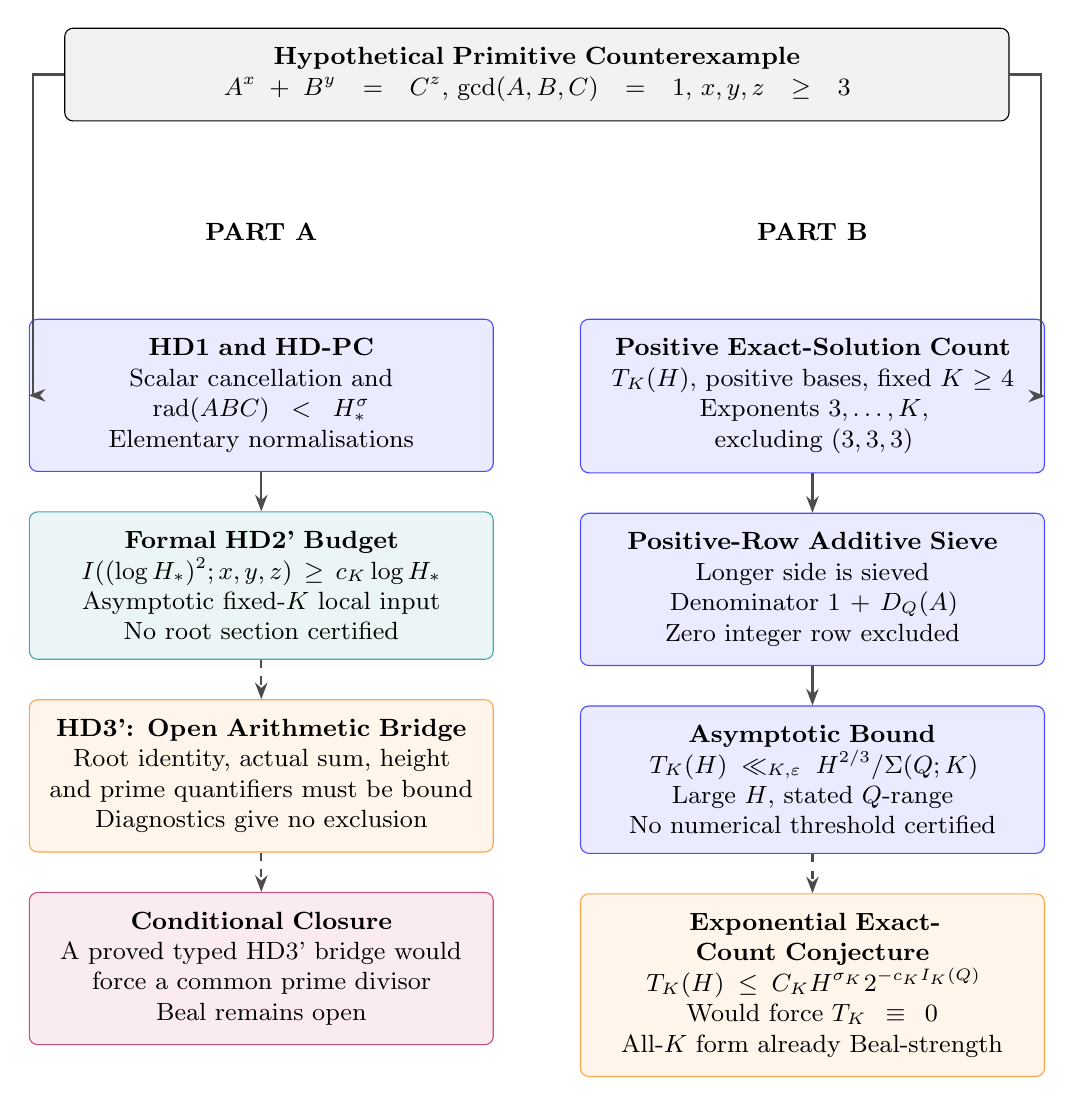
\begin{tikzpicture}[
 box/.style={rectangle,draw,rounded corners=3pt,align=center,
             text width=5.4cm,inner sep=7pt,font=\small},
 proven/.style={box,fill=blue!8,draw=blue!70},
 budget/.style={box,fill=teal!8,draw=teal!70},
 openbarrier/.style={box,fill=orange!8,draw=orange!70},
 closure/.style={box,fill=purple!8,draw=purple!70},
 arrow/.style={-{Stealth[length=6pt]},thick,draw=black!70},
 dasharrow/.style={arrow,dashed}
]
\node[box,text width=11.5cm,fill=gray!10] (input) at (0,1.3) {\textbf{Hypothetical Primitive Counterexample}\\$A^x+B^y=C^z$, $\gcd(A,B,C)=1$, $x,y,z\ge3$};
\node[align=center,font=\small\bfseries] at (-3.5,-0.7) {PART A};
\node[align=center,font=\small\bfseries] at (3.5,-0.7) {PART B};
\node[proven,anchor=north] (hd1) at (-3.5,-1.8) {\textbf{HD1 and HD-PC}\\Scalar cancellation and\\$\rad(ABC)<H_*^\sigma$\\Elementary normalisations};
\node[budget,below=0.5cm of hd1] (hd2) {\textbf{Formal HD2' Budget}\\$I((\log H_*)^2;x,y,z)\ge c_K\log H_*$\\Asymptotic fixed-$K$ local input\\No root section certified};
\node[openbarrier,below=0.5cm of hd2] (hd3) {\textbf{HD3': Open Arithmetic Bridge}\\Root identity, actual sum, height and prime quantifiers must be bound\\Diagnostics give no exclusion};
\node[closure,below=0.5cm of hd3] (closureA) {\textbf{Conditional Closure}\\A proved typed HD3' bridge would force a common prime divisor\\Beal remains open};
\node[proven,anchor=north] (count) at (3.5,-1.8) {\textbf{Positive Exact-Solution Count}\\$T_K(H)$, positive bases, fixed $K\ge4$\\Exponents $3,\ldots,K$, excluding $(3,3,3)$};
\node[proven,below=0.5cm of count] (sieve) {\textbf{Positive-Row Additive Sieve}\\Longer side is sieved\\Denominator $1+D_Q(A)$\\Zero integer row excluded};
\node[proven,below=0.5cm of sieve] (bound) {\textbf{Asymptotic Bound}\\$T_K(H)\ll_{K,\varepsilon}H^{2/3}/\Sigma(Q;K)$\\Large $H$, stated $Q$-range\\No numerical threshold certified};
\node[openbarrier,below=0.5cm of bound] (expheur) {\textbf{Exponential Exact-Count Conjecture}\\$T_K(H)\le C_KH^{\sigma_K}2^{-c_KI_K(Q)}$\\Would force $T_K\equiv0$\\All-$K$ form already Beal-strength};
\draw[arrow] (input.west) -- ++(-0.4,0) |- (hd1.west);
\draw[arrow] (input.east) -- ++(0.4,0) |- (count.east);
\draw[arrow] (hd1.south) -- (hd2.north);
\draw[dasharrow] (hd2.south) -- (hd3.north);
\draw[dasharrow] (hd3.south) -- (closureA.north);
\draw[arrow] (count.south) -- (sieve.north);
\draw[arrow] (sieve.south) -- (bound.north);
\draw[dasharrow] (bound.south) -- (expheur.north);
\end{tikzpicture}}
\caption{Conditional reduction (Part A) and asymptotic sieve companion (Part B). The formal entropy budget certifies no root coherence. The arithmetic bridge remains open; the polynomial count supplies no deterministic exclusion.}
\label{fig:bhd_architecture}
\end{figure}

\section{Conditional Closure}

\begin{theorem}[Height-Dominance closure, conditional]
\label{thm:conditional-closure}
Assume \cref{conj:hd3prime} for all exponent triples $x,y,z>2$, with
the $(3,3,3)$ case handled by Fermat's theorem for exponent~$3$. Then
Beal's conjecture holds.

The verifier-packet conjecture \cref{conj:hd2prime} is not a separate
logical assumption in this last implication. Its role is diagnostic and
constructive: it identifies the local information that any future proof
of \cref{conj:hd3prime} would have to transport beyond the CRT window.
\end{theorem}

\begin{proof}
Suppose a primitive Beal counterexample exists. By
\cref{lem:pairwise,prop:compression}, it lies in the power-radical
microcluster and satisfies $R < H_*^{\sigma}$. Since the equality is
exact, for every prime $q$ the residue $A^x+B^y \bmod q$ is a $z$-th
power, namely $C^z \bmod q$. Thus $V_q(A,B;x,y,z)=1$ for every $q$.
\Cref{conj:hd3prime} then forces a common prime divisor of $A,B,C$,
contradicting primitivity. Hence no primitive counterexample exists.
\end{proof}

\section{Approach to HD3': An Honest Sketch}
\label{sec:hd3-approach}

The deterministic route depends on HD3'. Restated: \emph{If
a primitive tuple $(A,B,C;x,y,z)$ in the power-radical microcluster
satisfies $V_q = 1$ for every prime $q$, then $\gcd(A,B,C) > 1$.}

\subsection*{What is known}

HD1 (\cref{lem:hd1}) is the scalar equation divided by $H_*=C^z$.
HD-PC (\cref{prop:compression}) is the elementary bound
$\rad(ABC)<H_*^\sigma$. These are normalisations, not arithmetic
exclusion. The existence form of HD2' (\cref{conj:hd2prime}) follows
asymptotically from the fixed-$K$ density and prime-progression inputs;
$Q=(\log H_*)^2$ suffices for large height. Its entropy depends on
the exponents and primes, not on the actual bases. The historical
near-misses are diagnostics and do not establish root coherence.

\subsection*{The hard barrier}

A pass says that $A^x+B^y$ has some $z$-th root modulo $q$;
it does not identify that root with the chosen $C$.
A valid global exclusion needs a precise contract relating the actual
sum, root identity, height and prime quantifiers. Statistical
independence of the congruence tests is not justified for the short
integer search box. Conversely, this paper proves no general
dependence theorem forcing a common prime divisor.
The polynomial bound of \cref{thm:sieve} does not give HD3'.
The exponential cumulative-count conjecture \cref{conj:exp} would
already imply Beal when formulated for every fixed exponent bound.

\subsection*{Tools that may apply}

Classical sieves supply the additive estimate in Part~B.
Averaging, short character sums, cyclotomic descent, and Frey/S-Unit
methods are candidate tools requiring a signature-specific transfer
and a uniformity check when fields or prime sets vary.
The fixed-signature finiteness theorem of Darmon--Granville
\cite{DarmonGranville1995} gives no general emptiness certificate.
No list of candidate methods constitutes an applicability theorem or
a proof that all possible transfers fail.

\subsection*{Concrete sub-goals and their corrected scope}
\begin{enumerate}[leftmargin=*]
\item \textbf{HD3'-RC / HD3'-A.} A finite root-coherence or salt-closing
contract must specify positive bases, the actual value $A^x+B^y$, a
common bounded integer root and the prime/height quantifiers. A large
formal root-capacity defect is not a deterministic obstruction on its
own. No strict implication hierarchy or uniform exclusion is certified.
\item \textbf{HD3'-B: weak input and rejected uniform strong form.}
For nontrivial $\eta$, all multiplicative characters extended by zero
at zero, put $H_x=\{\chi:\chi^x=1\}$ and
$J(\chi,\psi)=\sum_t\chi(t)\psi(1-t)$. The exact consolidation is
\[
 S_\eta(x,y;q)=(q-1)
 \sum_{\substack{\chi\in H_x\setminus\{1\},\,\psi\in H_y\setminus\{1\}\\
                 \chi\psi=\eta^{-1}}}J(\chi,\psi).
\]
The one-trivial-character terms cancel the axis contributions;
the factor $q-1$ must not be omitted. Classical Jacobi bounds
\cite[Ch.~8]{IrelandRosen} give the weak $O_K(q^{3/2})$ input.
For $q\equiv1\pmod{12}$, $(x,y)=(3,4)$ and $\eta$ of order $12$
there is one resonance pair, so
$|S_\eta|=(q-1)\sqrt q$. This refutes a blanket
$\eta$-uniform $q^{1+\varepsilon}$ bound for $\varepsilon<1/2$
even in a coprime mixed case. It does not refute restricted
$(3,4,5)$ statements.

The scalar family $a^x+b^y=c$ is constant after the finite étale
base change $c=t^L$ on $\mathbb G_m$, $L=\mathrm{lcm}(x,y)$:
$a=t^{L/x}u$, $b=t^{L/y}v$ reduces it to $u^x+v^y=1$.
In characteristic not dividing $xy$, its geometric monodromy factors
through a finite deck group; this particular family cannot have a
positive-dimensional full symplectic monodromy group.
No trivialisation at $c=0$, general Frey-family no-go or Xu-equivalence
\cite{Xu2020,FouvryKatz2001,KatzTwistedL} is inferred.
\item \textbf{HD3'-C / HD3'-D.} Counts of all local-pass tuples and
counts of exact positive solutions are different. No equivalence of
these counting/salt/cofactor goals with \cref{conj:exp} is proved.
\item \textbf{HD3'-E: external exact-solution result.}
Siksek--Stoll's Theorem 1.1 \cite{SiksekStoll2012} resolves the
primitive integer equation $u^3+v^4+w^5=0$ with only trivial solutions.
Putting $w=-C$ excludes positive primitive $A^3+B^4=C^5$.
It does not prove the proposed verifier statement for every local-pass
tuple with an unbound $C$, nor validate our architecture.
The corrected asymptotic sieve at $K=5$, $Q=H^{1/10}$ gives only
$T_{(3,4,5)}(H)\ll H^{29/60}\log H$; $Q=H^{1/5}$ is outside
the clean uniform range.
\end{enumerate}

\subsection*{What remains open}
HD3' and a typed low-root comparison remain open. The standard additive
sieve does not produce the proposed exponential cumulative count bound.
The latter is already Beal-strength under the formal entropy inputs,
as explained in \cref{conj:exp}. Failed candidate routes or restricted
source theorems prove no impossibility theorem for all methods.

\section{What Is Not Used}

No abc, Szpiro or Riemann-hypothesis implication is used to close Beal.
The Zookeeper comparison is architectural. A shared geometric or
operator setting for a Beal transfer has not been constructed here;
this absence is not a general impossibility theorem for a
Hilbert--Polya route or for common geometry.

\bigskip\hrule\medskip
\begin{center}
\textbf{Part B. Power-Residue Sieve Companion (Asymptotic Bound)}
\end{center}
\medskip\hrule\bigskip

\section{The Sieve Setup}
\label{sec:weilinput}

Part~B supplies a uniform asymptotic counting estimate for the finite
exponent box, on named classical inputs. It complements the
qualitative fixed-signature finiteness theorem
\cite{DarmonGranville1995}, but certifies no explicit height threshold.
The entropy table is historical descriptive evidence.
The exponential positive-count conjecture is already Beal-strength;
it is not an established weaker bridge to HD3'.

\section{Power-Residue Verifiers (Part~B)}

% TOOLBOX-NOTE: Character-sum techniques used throughout Part B
% (Jacobi sums, elementary boundary counts, Bombieri 1971 large sieve) are
% consolidated in FST_MATHEMATICS/_tools/CHARACTER_SUMS_TOOLBOX.md
% (Werkzeuge A, B, C, F). Bei Konsistenz-Reviews als Referenz nutzen.

Let $q$ be any prime and $z \ge 3$. Set
\[
  R_z(q) = \{u^z \bmod q : u \in \mathbb{F}_q\},
  \qquad
  |R_z(q)| = 1 + (q-1)/\gcd(z,q-1).
\]

\begin{definition}[Local acceptance density]
\label{def:delta}
For a prime $q$ with $\gcd(z,q-1)>1$ and exponents $x,y,z>2$,
\[
  \delta_q(x,y,z) :=
    \frac{|\{(a,b)\in \mathbb{F}_q^2 : a^x+b^y \in R_z(q)\}|}{q^2}.
\]
For trivial $q$ (i.e.\ $\gcd(z,q-1)=1$) the sieve gives no information,
so density and entropy sums retain only nontrivial primes.
\end{definition}

\begin{definition}[Verifier indicator]
\label{def:Vq}
For a tuple $(A,B,x,y,z)$ and any prime $q$,
\[
  V_q(A,B;x,y,z) :=
    \mathbf{1}\bigl\{(A^x+B^y) \bmod q \in R_z(q)\bigr\}.
\]
At trivial primes $\gcd(z,q-1)=1$, $R_z(q)=\mathbb F_q$ and
$V_q=1$. Density sums retain only nontrivial primes.
\end{definition}

\begin{lemma}[Necessary condition]
\label{lem:necessary}
If $(A,B,C;x,y,z)$ satisfies $A^x+B^y=C^z$, then
\[
  V_q(A,B;x,y,z)=1
\]
for every prime $q$.
\end{lemma}

\begin{proof}
$A^x+B^y \equiv C^z \pmod q$, and $C^z \bmod q \in R_z(q)$ by
definition.
\end{proof}

\begin{definition}[Cumulative verifier entropy]
\label{def:Iverifier}
For a verifier bound $Q$ and exponents $x,y,z>2$,
\[
  I(Q;x,y,z) := \sum_{q \le Q,\ \gcd(z,q-1)>1} -\log_2 \delta_q(x,y,z).
\]
\end{definition}

\section{Worst-Case Acceptance Density}

Fix an integer $K\ge4$. For every prime with a nonempty eligible
index set define
\[
 \delta_{q,K}^{*}=\max_{\substack{3\le x,y,z\le K\\
                         \gcd(z,q-1)>1}}\delta_q(x,y,z).
\]
Primes with an empty index set are omitted from sums using this
quantity; an empty maximum is not assigned a numerical value.

\begin{lemma}[Uniform character-sum bound for $\delta_q$]
\label{lem:weil}
For $3\le x,y,z\le K$, $q>K^4$, $q\nmid xyz$, and
$d=\gcd(z,q-1)>1$, the classical Jacobi-sum input gives
\[
 \left|\delta_q(x,y,z)-\frac1d\right|\le\frac{2K}{\sqrt q}.
\]
\end{lemma}

\begin{proof}
Write $H_m=\{\chi:\chi^m=1\}$ for multiplicative characters of
$\mathbb F_q^*$. Extend every character by zero at zero, including
the trivial character. Put $N_0=\#\{(a,b):a^x+b^y=0\}$ and
$S_\eta=\sum_{a,b}\eta(a^x+b^y)$. The power-residue indicator yields
the exact identity
\[
 q^2\delta_q=\frac{q^2}{d}
       +N_0(1-1/d)+\frac1d\sum_{\substack{\eta\in H_z\\\eta\ne1}}S_\eta.
\]
For $a=0$ only $b=0$ contributes to $N_0$; for $a\ne0$ there are
at most $K$ choices of $b$. Thus $N_0\le1+K(q-1)\le Kq$.

For nontrivial $\eta$, convolution and character orthogonality give
\[
 S_\eta=(q-1)
 \sum_{\substack{\chi\in H_x\setminus\{1\},\
                 \psi\in H_y\setminus\{1\}\\
                 \chi\psi=\eta^{-1}}}J(\chi,\psi).
\]
Indeed, the power-map fibre count is
$\sum_{\chi\in H_x}\chi(u)+\mathbf1_{\{u=0\}}$.
For $u+v=s\ne0$, substitution $u=st$, $v=s(1-t)$ leaves
$\sum_{s\ne0}(\chi\psi\eta)(s)$, which is zero except in resonance.
The resonant terms with one trivial character have Jacobi sum $-1$;
they cancel exactly against the corresponding axis contributions.
The pair with both characters trivial has no resonance because
$\eta\ne1$.

There are at most $K$ remaining resonant pairs, and their product
$\chi\psi=\eta^{-1}$ is nontrivial. The classical Jacobi-sum
identity gives $|J(\chi,\psi)|=\sqrt q$
\cite[Ch.~8]{IrelandRosen}. Therefore
$|S_\eta|\le K(q-1)\sqrt q$. Dividing the exact identity by $q^2$
gives an error at most $K/q+K/\sqrt q\le2K/\sqrt q$.
\end{proof}

\begin{remark}[Scope of the input]
The argument uses the named classical Jacobi-sum identity, with
the character and boundary conventions displayed above. It supplies
a local density estimate. It supplies neither a uniform
$q^{1+\varepsilon}$ bound for all twisted two-variable sums nor a
global exclusion theorem. Historical companion notes and their
review seals are retained as historical evidence.
\end{remark}

\begin{lemma}[Worst-case upper bound]
\label{lem:worstcase}
For eligible primes $q>K^4$,
\[
 \delta_{q,K}^{*}\le\frac12+\frac{2K}{\sqrt q}.
\]
\end{lemma}
\begin{proof}
For every eligible triple, $d\ge2$, so $1/d\le1/2$.
Apply \cref{lem:weil} and then take the maximum.
\end{proof}

\section{The Asymptotic Sieve Bound}
\label{sec:sieve}

\begin{theorem}[Uniform asymptotic sieve bound]
\label{thm:sieve}
Fix an integer $K\ge4$ and $\varepsilon>0$. Let $T_K(H)$ count
primitive tuples with \emph{positive integer} bases $A,B,C$,
$A^x+B^y=C^z$, $3\le x,y,z\le K$, $C^z\le H$, and
$(x,y,z)\ne(3,3,3)$. Define
\[
 \Sigma(Q;K)=
 \sum_{\substack{q\le Q\\
      \exists\,3\le z'\le K:\ \gcd(z',q-1)>1}}
       \frac{1-\delta_{q,K}^{*}}{\delta_{q,K}^{*}}.
\]
On the classical character-sum, additive large-sieve, and fixed-modulus
prime-number-theorem inputs specified below, for sufficiently large
$H$ and every
\[
 (\log H)^{2+\varepsilon}\le Q\le H^{1/(2K)}
\]
one has
\[
 T_K(H)\ll_{K,\varepsilon}\frac{H^{2/3}}{\Sigma(Q;K)}.
\]
The lower cut is sufficient, not necessary. This statement certifies
neither explicit implied constants nor an explicit numerical threshold
$H_0(K,\varepsilon)$ or a claimed order $K^{\Theta(K)}$.
\end{theorem}

\begin{remark}[Domain and parameter range]
For fixed $K,\varepsilon$ the displayed range is nonempty for large
$H$. Small heights admit the trivial positive-box bound; they are not
silently included in the asymptotic comparison. For $K=3$ the sole
triple is removed by the classical cubic Fermat case, and $T_3=0$;
no empty maximum is used. The uniform upper cut absorbs $Q^2$ into
the longer side of the search box.
\end{remark}

\begin{lemma}[Positive-row additive large sieve]
\label{lem:LS2}
For $M$ positive rows, let the variable in each row range over an
interval of $L$ consecutive integers. For every prime $q\le Q$ let
the allowed row classes have density $\delta_q(A)$, and put
\[
 D_Q(A)=\sum_{q\le Q}\frac{1-\delta_q(A)}{\delta_q(A)}.
\]
If an allowed set is empty, that row has no survivors. Otherwise
the total number of survivors is at most
\[
 \sum_{A=1}^{M}\min\left\{L,\
       \frac{L-1+Q^2}{1+D_Q(A)}\right\}.
\]
In particular the expression is defined when $D_Q(A)=0$.
\end{lemma}

\begin{proof}
Fix one row and let $Z$ be its survivor count. Write
$S(\alpha)=\sum_{n\ {\rm surviving}}e^{2\pi i n\alpha}$.
Parseval and Cauchy--Schwarz on the allowed residue classes yield
\[
 \sum_{a=1}^{q-1}|S(a/q)|^2
       \ge Z^2\frac{1-\delta_q(A)}{\delta_q(A)}.
\]
The frequency zero and the reduced fractions $a/q$ for distinct
primes are distinct modulo one and $Q^{-2}$-separated.
The classical additive large sieve
\cite{Bombieri1971,KedlayaANT} therefore gives
\[
 Z^2(1+D_Q(A))\le(L-1+Q^2)Z.
\]
For $Z>0$ divide by $Z$; for $Z=0$ the conclusion is immediate.
Also $Z\le L$. Sum over the positive rows. The precise additive
input is stated in \cite[Theorem~18.1]{KedlayaANT}.
\end{proof}

\begin{remark}[Row densities and comparison with $\Sigma$]
\label{rem:Sigma-comparison}
For the classes $a^x+b^y\in R_z(q)$ put $d_y=\gcd(y,q-1)$,
$d_z=\gcd(z,q-1)$. The zero-residue row has the exact density
\[
 \delta_q(0)=
 \frac{1+(q-1)\gcd(d_y,d_z)/d_z}{q}.
\]
Thus $\delta_q(0)=1$ exactly when $d_z\mid d_y$.
For example $q=7,y=3,z=6$ gives $4/7$, whereas $y=6,z=3$ gives $1$.

For $a\ne0$ and $q\nmid y$, the polynomial $a^x+b^y$ is squarefree.
The classical one-variable multiplicative character bound gives
\[
 \left|\delta_q(a)-\frac1{d_z}\right|\le2Kq^{-1/2}.
\]
Here the zeros of the polynomial contribute at most $K/q$, and the
nontrivial character sums contribute at most $K/\sqrt q$.
Consequently, for \emph{nontrivial} primes $d_z>1$ and
$q>144K^2$, $\delta_q(a)\le2/3$ and the sieve weight is at least
$1/2$. At trivial primes $d_z=1$, the density is $1$ and the weight
is zero; those primes must not be used for this lower bound.

For a positive integer row $A$, only its prime divisors have
$A\bmod q=0$. With
$\pi_z(Q)=\#\{q\le Q:\gcd(z,q-1)>1\}$, this gives
\[
 D_Q(A)\ge
 \tfrac12\{\pi_z(Q)-\omega(A)-\pi(144K^2)\}.
\]
The row $A=0$ is excluded; $\omega(0)$ is not defined.
The elementary bound $\omega(A)\le\log_2 H$ for $1\le A\le H$
is sufficient here, but not asymptotically sharp: if $\omega(A)=k$,
then $A\ge(k+1)!$, yielding
$\omega(A)=O(\log H/\log\log H)$.

For fixed $3\le z\le K$, primes $q\equiv1\pmod{\ell}$ for a prime
divisor $\ell$ of $z$ are nontrivial for $z$.
The fixed-modulus prime number theorem in arithmetic progressions
\cite[Theorem~4.12]{KedlayaANT} gives
$\pi_z(Q)\asymp_K Q/\log Q$ as $Q\to\infty$.
The row denominator uses this \emph{fixed-$z$} prime count, not the
larger union of eligible primes for different $z'$.
For $K\ge4$, $z'=4$ makes every odd prime eligible, and
\cref{lem:weil,lem:worstcase} imply
$\Sigma(Q;K)\asymp_K Q/\log Q$: for large primes each local
density lies between a positive $K$-dependent constant and $2/3$;
the finitely many smaller primes have finite weights.

The sufficient lower cut in \cref{thm:sieve} therefore makes
$\pi_z(Q)$ dominate $\log_2 H+\pi(144K^2)$ uniformly in the
positive rows, for sufficiently large $H$. No comparison with the
upper endpoint $H^{1/(2K)}$ is substituted for the actual $Q$.
The lower cut is not a necessary condition or an equivalence.
If $Q$ grows below that cut, $\Sigma(Q;K)$ need not remain bounded;
an averaged extension to that range is not established here.
\end{remark}

\begin{proof}[Proof of \cref{thm:sieve}]
Fix an eligible exponent triple and put
$U=H^{1/\min(x,y)}$, $V=H^{1/\max(x,y)}$.
The positive $(A,B)$ box has its longer side at most $U$ and its
shorter side at most $V$. Transpose the variables when necessary:
the shorter side indexes the positive rows and the longer side
is sieved. The row-density argument in
\cref{rem:Sigma-comparison} applies with $x,y$ interchanged as needed.

Throughout the stated range, for large $H$ every positive row has
$D_Q(A)\gg_K Q/\log Q\asymp_K\Sigma(Q;K)$.
Also $Q^2\le H^{1/K}\le U$.
Taking $L=\lfloor U\rfloor$ and $M=\lfloor V\rfloor$ in
\cref{lem:LS2} bounds the survivor pairs by
\[
 \ll_K\frac{UV}{\Sigma(Q;K)}
       =\frac{H^{1/x+1/y}}{\Sigma(Q;K)}.
\]
Each positive pair has at most one positive integer $C$ satisfying
$C^z=A^x+B^y$; retaining only primitive pairs and the condition
$C^z\le H$ can only decrease the count. Since $1/x+1/y\le2/3$,
summing over finitely many exponent triples gives the stated
$\ll_{K,\varepsilon}$ bound. All implied constants are retained;
the proof does not replace an asymptotic inequality by an exact
coefficient-one inequality.
\end{proof}

\begin{remark}[Exceptional primes and the unabsorbed remainder]
\label{rem:exceptional}
For fixed $K$, omitting the finitely many small primes or primes
dividing $xyz$ removes $O_K(1)$ total weight; no assertion that
each individual weight is at most one is needed.
For a fixed triple, under the same sufficient lower cut and
large-height condition, the unabsorbed row estimate is
\[
 T_{(x,y,z)}(H)\ll_K
 \frac{H^{1/x+1/y}+H^{1/\max(x,y)}Q^2}{\Sigma(Q;K)}.
\]
The uniform upper cut in the theorem absorbs the second term.
Explicit constants, a certified numerical height threshold, and
an extension to smaller growing sieve ranges remain separate tasks.
\end{remark}

\section{Empirical Verification}
\label{sec:empirical}

The historical 1000-row near-miss table reports four nested
verifier bounds. Its values are reproduced as descriptive diagnostics;
the local-density asymptotic is a separate mathematical input.

\begin{table}[htb]
\centering
\begin{tabular}{rrrr}
\toprule
$Q$ & $I(Q)$ median (bits) & $I(Q)/\pi(Q)$ & slope$_{\min}$ vs.\ $\log H_*$ \\
\midrule
$251$  & $38.24$  & $0.71$ & $+0.704$ \\
$503$  & $69.78$  & $0.73$ & $+1.116$ \\
$1009$ & $126.70$ & $0.75$ & $+1.737$ \\
$2003$ & $232.75$ & $0.77$ & $+4.289$ \\
\bottomrule
\end{tabular}
\caption{Historical reported verifier entropy for 1000 near-misses with $\log H_*\in[16,39]$. The four nested bounds give descriptive ratios and slopes. They establish neither convergence, statistical significance nor independent method validation.}
\label{tab:emp}
\end{table}

\begin{remark}[Descriptive status]
The table reproduces historical reported values without a new run.
The formal fixed-$K$ entropy budget follows from classical local
inputs and is independent of the bases. Neither the table nor its
nested prime bounds supply a significance test, a root section,
an exponential survivor bound or HD3'.
\end{remark}

\begin{remark}[Root-coherence guardrail]
The verifier $V_q(A,B;x,y,z)$ is deliberately a coarse pass/fail
condition: it asks whether some local $z$-th root exists modulo $q$.
An exact Beal closure requires more. The same small integer $C$ must
reduce to compatible local roots for all primes under consideration.
Equivalently, for
\[
  R_q(A,B)=\{c\in\mathbb F_q:\ c^z\equiv A^x+B^y\pmod q\},
\]
one needs a low-height global section $C\le H^{1/z}$ through the local
sets $R_q(A,B)$, not merely the non-emptiness of each set. The empirical
entropy table therefore supports only the pass/fail verifier layer. A
future HD3' route would need to keep track of root identity, for instance via the
root-coherence capacity framework recorded in the companion proof notes.
The June 2026 S-Unit/Frey shadow and Q97-plus synthetic-control audits
sharpen the same requirement: Q97-plus local survival alone is never
evidence. A future survivor may be read as stronger only if it is
Q97-plus, branch-bound from the actual value $A^x+B^y$, and accompanied
by a low-height global root section or source-bound S-Unit/Frey data.
\end{remark}

\begin{table}[htb]
\centering
\small
\begin{tabularx}{\textwidth}{@{} >{\raggedright\arraybackslash}p{0.20\linewidth} >{\raggedright\arraybackslash}p{0.25\linewidth} >{\raggedright\arraybackslash}p{0.22\linewidth} >{\raggedright\arraybackslash}X @{}}
\toprule
Diagnostic layer & Sample and range & Observed signal & Interpretation \\
\midrule
Verifier entropy & 1000 near-misses, $Q\in\{251,503,1009,2003\}$ &
$I(Q)/\pi(Q)=0.71$--$0.77$ &
Historical descriptive scaling; no root-coherence validation. \\
\addlinespace
Rough root pilot & 250 near-misses, $Q\in\{251,503,1009\}$ &
$250/250$ empty actual root sets; exact-power control $250/250$ &
Local obstruction appears before root drift; the control checks detector sanity. \\
\addlinespace
Small-block survivor scan & 250 near-misses, $Q\in\{7,13,31,61\}$ &
one drift-without-section case at $Q=31$; all actual rows fail locally by $Q=61$ &
The drift zone is finite and transitional in this sample. \\
\addlinespace
Above-threshold scan & 5000 near-misses, checkpoints $31$--$127$ &
five $Q=61$ passes without low section; $0/5000$ local passes at $Q=97$ &
No stable above-threshold survivor; follow-up gates must use source-bound families and controls. \\
\addlinespace
S-Unit/Frey shadow audit & five $Q=61$ survivors, June 2026 &
$0$ Q97-plus survivors; $0$ direct S-Unit/Frey anchors &
Only method-shadow context remains; no source-bound support for HD3'. \\
\addlinespace
Q97-plus synthetic controls & natural survivors plus registered, shifted, and shuffled controls &
natural $0/5$ Q97-plus; controls reach $Q=127$ only through synthetic sections or branch maps &
Local pass aggregates alone are negative controls; the triple gate is mandatory. \\
\bottomrule
\end{tabularx}
\caption{Root-coherence and verifier diagnostic ledger. The rows separate
evidence for the additive verifier layer from tests probing low-height
root sections. All root-coherence rows are internal diagnostics, not
proof evidence for HD3'.}
\label{tab:root-diagnostics}
\end{table}

\section{The Stronger Conjecture}

\begin{definition}[Uniform box exponent and entropy]
\label{def:sigmaK}
For an integer $K\ge4$ define
\[
 \sigma_K=\max_{\substack{3\le x,y,z\le K\\(x,y,z)\ne(3,3,3)}}
                       (1/x+1/y)=2/3,\qquad
 I_K(Q)=\min_{\substack{3\le x,y,z\le K\\(x,y,z)\ne(3,3,3)}}
                       I(Q;x,y,z).
\]
These index sets are finite and nonempty; no $K=3$ maximum is used.
The exponent is the ceiling of the particular positive-box estimate
in \cref{thm:sieve}, not a ceiling theorem for all arithmetic methods.
The local-density and fixed-progression inputs imply
$I_K(Q)\gg_K Q/\log Q$ for large $Q$.
\end{definition}

\begin{conjecture}[Exponential cumulative-count bound]
\label{conj:exp}
For each fixed integer $K\ge4$ there exist constants $a_K\ge2$,
$c_K>0$ and $C_K>0$ such that, for sufficiently large $H$ and
$Q=(\log H)^{a_K}$,
\[
 T_K(H)\le C_K H^{\sigma_K}2^{-c_K I_K(Q)}.
\]
The count is the cumulative positive primitive exact-solution count
defined in \cref{thm:sieve}, not a count of local-pass pairs.
\end{conjecture}

\begin{remark}[Why this is already Beal-strength]
The logarithm of the right side is at most
\[
 \sigma_K\log H-c'_K
       \frac{(\log H)^{a_K}}{\log\log H}+O_K(1)\longrightarrow-\infty.
\]
Thus the bound forces $T_K(H)<1$ for all sufficiently large $H$.
Since $T_K$ is nonnegative, integer-valued and nondecreasing,
it follows that $T_K(H)=0$ at \emph{every} height.
For all fixed $K$ this excludes every positive primitive mixed
signature, with the cubic signature excluded classically.
Conversely, Beal makes all these counts zero and hence makes the
displayed bound immediate. Under the stated entropy inputs the
all-$K$ formulation therefore has Beal strength.

A product of densities is exact for a complete CRT residue domain;
it is not automatically a survivor probability in a short box.
Independence beyond that window is not justified here.
No equivalence with a conjecture for local-pass pairs or a strict
hierarchy of root-coherence subgoals is asserted.
\end{remark}

\section{The CRT Product Window}
\label{sec:crt-window}

The multiplicative product heuristic is not false in every range. It is
exact in the finite Chinese-remainder window, and this exact statement
explains where the barrier begins.

\begin{lemma}[CRT product window]
\label{lem:crt-window}
Let $P$ be a finite set of primes and let $M(P)=\prod_{q\in P}q$.
For each $q\in P$, let $S_q\subseteq\mathbb F_q^2$ and put
$\delta_q=|S_q|/q^2$. Let $S_M\subseteq(\mathbb Z/M(P)\mathbb Z)^2$
be the CRT product of the $S_q$. Then
\[
  |S_M|=M(P)^2\prod_{q\in P}\delta_q.
\]
If $N_P(X,Y)$ counts pairs $(A,B)\in[1,X]\times[1,Y]\cap\mathbb Z^2$
whose residue class modulo $M(P)$ lies in $S_M$, then
\[
  N_P(X,Y)
  = XY\prod_{q\in P}\delta_q
    + O\!\left(\prod_{q\in P}\delta_q\,
      (M(P)X+M(P)Y+M(P)^2)\right).
\]
In particular, relative product asymptotics hold whenever
$M(P)=o(\min(X,Y))$.
\end{lemma}

\begin{proof}
The CRT identifies $(\mathbb Z/M(P)\mathbb Z)^2$ with
$\prod_{q\in P}\mathbb F_q^2$, which gives the exact cardinality of
$S_M$. Each admissible residue class modulo $M(P)$ has
$XY/M(P)^2+O(X/M(P)+Y/M(P)+1)$ representatives in the box. Multiplying
by $|S_M|$ gives the stated formula.
\end{proof}

For the Beal verifier boxes one has $X=H^{1/x}$ and $Y=H^{1/y}$.
Thus the direct CRT product window requires
\[
  M(P)\ll H^{\min(1/x,1/y)}.
\]
For $P=\{q\le Q\}$, $\log M(P)=\vartheta(Q)\sim Q$, so this direct
window reaches only
\[
  Q\lesssim \min(1/x,1/y)\log H.
\]
In that maximal range the product of local densities gives at most a
subpolynomial gain of the shape $\exp(-c\pi(Q))=H^{-c/\log\log H+o(1)}$.
The desired regime $Q=(\log H)^A$ with $A>1$ already has
$M(P)=\exp((\log H)^A)$, far larger than the ordinary search box.

Consequently, the obstruction behind \cref{conj:exp} is not merely a
missing local character-sum improvement. It is the problem of
transporting product information beyond the CRT fundamental domain,
for example by bilinear dispersion, Frey-family geometry, Selmer or
Mordell--Weil structure, or a genuinely new correlation theorem.

\section{Comparison with Darmon--Granville}

Darmon--Granville \cite{DarmonGranville1995} establishes qualitative
finiteness of primitive solutions for each fixed hyperbolic
signature. Finiteness does not establish emptiness.
Part~B instead supplies the positive-box counting estimate
\cref{thm:sieve}, uniform over the finite exponent box for fixed $K$
and sufficiently large height, on the stated classical inputs.
It does not supply an explicit constant or certified numerical height
threshold. No effectivity advantage over the fixed-signature theorem
is claimed without that additional work. The signature classification
in \cref{tab:regime_matrix} does not itself construct a smooth cover
or determine its genus.

\section{Outlook: Bounded Negative Tests and Open Transfers}
\label{sec:outlook}

The following are candidate-method diagnostics, not general
impossibility theorems and not an independent proof of Beal.

\subsection{Strong twisted-sum claims and the additive estimate}
\label{sec:outlook-elim1}

The mixed $(3,4)$ resonance example in \cref{sec:hd3-approach}
invalidates a blanket $q^{1+\varepsilon}$ estimate for every
nontrivial character when $\varepsilon<1/2$.
It does not invalidate every character-restricted estimate for a
specific signature such as $(3,4,5)$.
The weaker estimate in \cref{lem:weil} suffices for the additive
bound. Improving local sums alone does not supply the missing
beyond-CRT transport in \cref{conj:exp}.
Historical attempts with Selberg weights, bilinear dispersion,
Heath-Brown identities and Halasz-type bounds
\cite{BFI1986,HB1982,HalaszPretentious} record unsuccessful transfers
within the tested formulations. They prove no universal second-order
parity barrier or exclusion of all standard sieve methods.

\subsection{Detection, counting and the cubic case}
\label{sec:outlook-elim2}

Prime-detection theorems for polynomial values
\cite{FI1998a,FI1998b,HB2001,HBMoroz2002,Merikoski2022} cannot be
imported as exact-solution counting results without a typed reduction.
The factorisation $A^3+B^3=(A+B)(A^2-AB+B^2)$ prevents a direct use
of a hypothesis requiring an irreducible cubic form; it does not
prove categorical incompatibility of detection and counting.
The positive primitive $(3,3,3)$ case is excluded by classical
Fermat for exponent three. Since its count is zero, any upper bound
with a nonnegative right side is automatically valid; it is
incorrect to say that descent cannot provide such an upper bound.
No unbound variable-count threshold is used as a general no-go theorem.

\subsection{Signature classification and its limits}
\label{sec:outlook-phase}

The sign of $\chi=1/x+1/y+1/z-1$ classifies orbifold signatures.
In the domain $x,y,z\ge3$, the only zero case is $(3,3,3)$;
the other cases are hyperbolic. Outside that domain,
$(2,2,z)$ is spherical, since $\chi=1/z>0$.
The sign alone does not establish parametric primitive families,
an exact smooth-cover genus, sieve applicability or emptiness.
Darmon--Granville gives fixed-hyperbolic-signature finiteness.
Selmer's diagonal-cubic examples \cite{Selmer1951} are a warning
about local-global transfer, not a theorem about the Fermat cubic.

\subsection{A typed beyond-CRT research question}
\label{sec:outlook-rqprime}

Can one transfer the product information in \cref{lem:crt-window}
to a specified short-box count by a proved correlation theorem?
A proposed Frey, Selmer, determinant-method or geometric-sieve route
\cite{BS2015,Bhargava2014,HeathBrown2002,KoymansSmith2024}
must name its objects, map, height comparison, multiplicity bound,
family restrictions and uniform constants. No automatic transfer
from those cited frameworks to general mixed Beal signatures is
established here. In particular, neither a universal $H^{2/3}$ roof
nor a sufficient Sato--Tate/Lang--Trotter implication is proved.
For the cumulative exact count, the exponential target is already
Beal-strength; for a local-pass count it is a different conjecture.

The most recent internal root-coherence notes sharpen this empirical
step into a rough-modulus root-coherence test. The diagnostic does not
merely count local pass/fail events; it separates small-prime
obstructions, rough-modulus density of the root sets $R_q(A,B)$,
unit/valuation/branch coherence, and the remaining noncoherent tail.
This is an experimental ledger, not a theorem. Its purpose is to make
visible whether a low-height global root section fails because of
ordinary local obstructions, insufficient rough-modulus density, or a
genuinely nonlocal coherence defect.

A limited internal pilot of this ledger on May~22, 2026, using $250$
near-miss rows and $Q\in\{251,503,1009\}$, found local obstruction
before drift in all actual near-miss cases: for each of the three prime
blocks, $250/250$ actual near-misses had an empty local root set and
$0/250$ low-height sections survived. June 2026 follow-up audits did
not reverse that negative pattern. The S-Unit/Frey shadow audit found
$0$ Q97-plus survivors and $0$ direct source-bound S-Unit/Frey anchors
among the five natural $Q=61$ survivors. The Q97-plus synthetic-control
audit showed that local Q97-plus or $Q=127$ pass aggregates can be
manufactured by registered sections or shuffled branch maps, but those
controls break branch binding or the low global section. This does not
close HD3'. It changes the next empirical task: a positive survivor
must satisfy all three gates at once--Q97-plus local survival, actual
branch binding from $A^x+B^y$, and a low global root section or
source-bound S-Unit/Frey data--before it can be read as more than a
diagnostic stress test.

\begin{remark}[Status of the research question]
These historical tests supply a bounded diagnostic ledger.
They neither certify HD3' nor rule out all alternative methods.
The corrected additive theorem retains precisely the domain and
large-height conditions of \cref{thm:sieve}.
\end{remark}

\section{Conclusion and Honest Status}

HD1 and HD-PC are elementary normalisations. The formal fixed-$K$
HD2' budget follows asymptotically from the stated classical local
inputs and does not certify root identity or global exclusion.
HD3' remains open and requires a typed root/height/prime contract.
The local density proof, positive-row additive sieve and
fixed-progression estimate give \cref{thm:sieve} only in its stated
large-height domain. No explicit constant package or certified
numerical threshold is supplied.
The exponential bound for the cumulative positive primitive exact
count would force the count identically to zero; its all-$K$
formulation is already Beal-strength.
Historical numerical tables, fitted scores, hard-coded gates and
source-file hash matches provide no additional exclusion theorem.
This corrective version does not promote the historical claim
register, certify an external computational proof, or establish a
general impossibility theorem for alternative methods.

\section{Corrective Inventory Note for Version 1.1}
\label{sec:inventory-corrections}

This section records the scope of the R25 inventory corrections.
It separates elementary identities, historical diagnostics,
source-reported literature and still-open arithmetic transfers.
Original producer files, result tables, claim statuses and historical
review seals are not rewritten by this manuscript revision.

\subsection{Elementary height identities and diagnostic gates}
For an exact positive sum $U+V=H$, put $u=U/H$ and
\[
 \Xi=\log\frac{H^2}{UV}=-\log[u(1-u)]\ge\log4,\qquad
 \Delta=\Xi-\log2\ge\log2.
\]
These inequalities are elementary and hold for nonprimitive exact
tuples as well. Fixed unequal proportions do not make $\Xi$ diverge;
divergence needs $\min(U,V)/H\to0$.
The exact family $(A,B,C;x,y,z)=(3t^5,6t^5,3t^3;3,3,5)$,
$t\ge1$, has $u=1/9$ and constant $\Xi$, and is nonprimitive.
It is no Beal counterexample.
An IUT/max-hull or gcd exclusion requires a separate, presently
missing arithmetic bridge; the elementary $\Delta$ inequality does
not provide it. A term defined as $\log H\,|\chi|$ grows by its
definition, not because an arithmetic obstruction was established.

The August/September diagnostic formula
$S_{\rm PH}=-\sum_q (1/q)/(1+\phi_q^2)$ is negative for every
nonempty prime set and every real input $\phi_q$.
Its sign cannot distinguish a primitive counterexample.
The historical branch-binding gate is a constant true flag, not
an implemented binding check. The historical survivor predicate
uses primitivity, exponent scope and exactness; it does not consume
the three diagnostic gates. Its zero survivor count therefore
does not validate the proposed exclusion mechanism.

The 25-row historical replay contains eleven primitive
in-scope rows: two parabolic $(3,3,3)$ rows and nine hyperbolic
rows. The named ten-row hyperbolic-primitive group contains one
parabolic row. One of five anchored controls has exponent two
and is not exact. Accordingly $0/11$, $0/10$ and $4/5$ are
different denominators and scopes, not interchangeable success
certificates. Nested prime bounds reuse observations; an
$\eta$-coefficient of variation is descriptive, not a replicated
experiment, confidence interval or significance test.

\subsection{The July function and provenance boundary}
The separate July diagnostic has the form
\[
 F(w)=\sum_{q,r}\frac{a_{q,r}}{w-e^{2\pi i r/q}},
 \qquad a_{q,r}>0,
\]
over nonempty root sets. One off-pole evaluation at
$w=0.5+0.5i$ does not establish the Herglotz property, which requires
holomorphy on the upper half-plane.
For the exact nonprimitive control $2^3+2^3=2^4$ the roots modulo
five include $r=1,2,3,4$, giving upper-half-plane poles with positive
residues that do not cancel. This invalidates that Herglotz claim;
it does not transfer the separate August sign argument to July.

The inventory found five PDF hashes matching the JSON validation
manifest and the checked local files, but conflicting hash fields
in the companion Markdown validation note. A local byte-identity
check is neither an external provenance audit nor a proof review.
Historical files and seals remain preserved; this corrective text
does not silently reseal them.

\subsection{Bounded literature update}
Chocian's preprint \cite{Chocian2026} reports a computer-assisted
exclusion of nonzero coprime integer solutions of signature
$(3,5,7)$. Its arXiv identity is confirmed. Its proof and replay
companion have not been independently validated here, and it does
not certify this paper's general verifier architecture.

Sahoo \cite[Theorem~1.10, Proposition~1.12]{Sahoo2026} is conditional
on Conjectures~2.4 and~2.5: for squarefree $d\ge5$,
$-d\not\equiv1\pmod8$, coefficients $\{\pm2^r\}$ and the source's
$\alpha_{\mathfrak p}\beta_{\mathfrak p}\gamma_{\mathfrak p}\ne0$,
it excludes sufficiently large \emph{common prime} exponents in
$W_{L,\mathfrak p}$, where $L=\mathbb Q(\sqrt{-d})$,
$\mathfrak p\mid2$ and $\mathfrak p\mid abc$.
The density $5/6$ is relative to squarefree $d$.
This is source-reported scope, not a general mixed-exponent HD3'
theorem or a uniform tower/coercivity estimate.

Pasten \cite[Corollaries~1.2--1.3]{Pasten2026} reports
$h(E)\ll N\log\log N$ for elliptic curves over $\mathbb Q$ and
$h(E)\ll_S N$ for curves semistable outside fixed $S$.
These statements concern the source's Faltings height and conductor.
They neither establish Szpiro's conjecture nor automatically remove
modular forms in a Beal transfer. The required uniform height and
S-Unit comparisons when prime sets or fields vary remain open.

\appendix

\section{Empirical data and reproducibility}
\label{app:data}

The historical 5000-row near-miss corpus was generated by
\path{evidence/scan_near_power_fractures.py} with
\texttt{--max-base 250}, \texttt{--min-exp 3}, \texttt{--max-exp 7} and
\texttt{--keep 5000}, \texttt{--max-rel-gap 1e-4}. The variable-$Q$ experiment
retains the first 1000 rows, ordered by relative gap, and uses
\path{evidence/run_variable_Q_sieve.py} for
$Q\in\{251,503,1009,2003\}$. Its recorded runtime of about 14 minutes
on a two-core server is historical, not a new benchmark.

The curated Beal source and data package is available at
\url{https://github.com/research-line/functional-stability-theory/tree/codex/beal-inventurernte-v1.1/fst-mathematics/beal-height-dominance}.
It contains both manuscript sources, the disclosure inputs, eight
historical diagnostic scripts, and 17 unchanged CSV files. The package
README documents the dataset selection, control classes, replay commands,
and claim limits. Its manifest binds the supplied artifacts by SHA-256;
the accompanying tests check artifact integrity and the reported finite
diagnostic summaries, not a proof of Beal's conjecture.

The May~22 root-branch-drift pilot supplies three 750-row ledgers:
250 actual near-misses, 250 random-root controls, and 250 exact-power
controls for each $Q\in\{251,503,1009\}$. The June~1 follow-up uses
$Q\in\{7,13,31,61\}$ on the same 250-row selection and the same three
control classes. The June~2 rank-8 micro-audit identifies the first
empty cubic-root channel at $q=37$; the 5000-row above-threshold scan
has five local passes at $Q=61$ and none at $Q=97$.
The June~22 S-unit-shadow and June~23 synthetic-control tables are
included as historical classifications. Synthetic registered, shifted,
or shuffled sections are controls and cannot establish branch binding
to the original arithmetic equation.
These files support the descriptive audit trail in
\cref{tab:root-diagnostics}; they do not establish HD3', root coherence,
statistical significance, or an effective height threshold. Internal
proof and review notes and third-party source PDFs are not part of
the public package.

% =============================================================================
% AI DISCLOSURE -- PIPELINE STANDARD, ENGLISH VERSION (since 2026-08-17, T-20260817-02)
% =============================================================================
% Language-pure version for English-only manuscripts. Text copied verbatim
% from the English block of ai_disclosure_STANDARD.tex (no content change) --
% only the heading is now language-pure and the German block is dropped. The
% bilingual file ai_disclosure_STANDARD.tex remains unchanged (existing
% references may keep pointing to it).
%
% DEVIATING DOWNWARD: If a paper genuinely used substantially less AI, do NOT
% switch to a different file -- weaken the wording here instead, e.g. replace
% "extensively in all phases" with the phases that actually applied, and
% strike whatever did not happen from the quality-assurance list. Principle:
% state honestly what happened -- do not hedge.
%
% Usage (English-only manuscripts only):
%   \input{../../_templates/disclosure/ai_disclosure_STANDARD_en}
% =============================================================================

\section*{AI Disclosure}

\noindent
AI systems were used extensively in all phases of this work: conception
and research discussion, literature and source work, mathematical analysis
and proof development, creation and checking of the computational scripts,
execution and evaluation of the computational runs, text, translation, and
typesetting.

\medskip

\noindent
Quality assurance: use of several independent models from different
providers with counter-checks and adversarial AI reviews; traceable,
versioned computational scripts with stored result files and checksums;
continuously maintained proof and register documents; strict claim hygiene
(assertions only with documented evidence, addenda instead of silent
corrections); changelogs across all versions.


\begingroup
\small
\setlength{\itemsep}{0pt}
\setlength{\parskip}{0pt}
\setlength{\parsep}{0pt}
\begin{thebibliography}{99}

\bibitem{BFI1986}
E.~Bombieri, J.~B.~Friedlander, and H.~Iwaniec, ``Primes in arithmetic
progressions to large moduli,''
\emph{Acta Mathematica} 156 (1986), 203--251. doi:
\href{https://doi.org/10.1007/BF02399204}{10.1007/BF02399204}.

\bibitem{Bhargava2014}
M.~Bhargava, ``The geometric sieve and the density of squarefree values
of invariant polynomials,'' arXiv:1402.0031 (2014).
\url{https://arxiv.org/abs/1402.0031}.

\bibitem{Bombieri1971}
E.~Bombieri, ``A note on the large sieve,''
\emph{Acta Arithmetica} 18 (1971), no.\ 1, 401--404. doi:
\href{https://doi.org/10.4064/aa-18-1-401-404}{10.4064/aa-18-1-401-404}.

\bibitem{BS2015}
M.~Bhargava and A.~Shankar, ``Binary quartic forms having bounded
invariants, and the boundedness of the average rank of elliptic
curves,'' \emph{Annals of Mathematics} 181 (2015), 191--242.
doi: \href{https://doi.org/10.4007/annals.2015.181.1.3}{10.4007/annals.2015.181.1.3};
arXiv:1006.1002.

\bibitem{DarmonGranville1995}
H.~Darmon and A.~Granville, ``On the equations $z^m=F(x,y)$ and
$Ax^p+By^q=Cz^r$,''
\emph{Bulletin of the London Mathematical Society} 27 (1995),
no.\ 6, 513--543. doi:
\href{https://doi.org/10.1112/blms/27.6.513}{10.1112/blms/27.6.513}.

\bibitem{FI1998a}
J.~B.~Friedlander and H.~Iwaniec, ``The polynomial $X^2+Y^4$ captures
its primes,'' \emph{Annals of Mathematics} 148 (1998), 945--1040.
doi: \href{https://doi.org/10.2307/121034}{10.2307/121034};
arXiv:math/9811185.

\bibitem{FI1998b}
J.~B.~Friedlander and H.~Iwaniec, ``Asymptotic sieve for primes,''
\emph{Annals of Mathematics} 148 (1998), 1041--1065.
doi: \href{https://doi.org/10.2307/121035}{10.2307/121035};
arXiv:math/9811186.

\bibitem{FouvryKatz2001}
\'E.~Fouvry and N.~M.~Katz, ``A general stratification theorem for
exponential sums, and applications,''
\emph{Journal f\"ur die reine und angewandte Mathematik (Crelle)}
540 (2001), 115--166. doi:
\href{https://doi.org/10.1515/crll.2001.082}{10.1515/crll.2001.082}.

\bibitem{HalaszPretentious}
G.~Hal\'asz, ``\"Uber die Mittelwerte multiplikativer zahlentheoretischer
Funktionen,'' \emph{Acta Mathematica Academiae Scientiarum Hungaricae}
19 (1968), no.\ 3--4, 365--403. doi:
\href{https://doi.org/10.1007/BF01894515}{10.1007/BF01894515}.

\bibitem{HB1982}
D.~R.~Heath-Brown, ``Prime numbers in short intervals and a
generalized Vaughan identity,''
\emph{Canadian Journal of Mathematics} 34 (1982), no.\ 6, 1365--1377.
doi: \href{https://doi.org/10.4153/CJM-1982-095-9}{10.4153/CJM-1982-095-9}.

\bibitem{HB2001}
D.~R.~Heath-Brown, ``Primes represented by $x^3+2y^3$,''
\emph{Acta Mathematica} 186 (2001), no.\ 1, 1--84. doi:
\href{https://doi.org/10.1007/BF02392715}{10.1007/BF02392715}.

\bibitem{HBMoroz2002}
D.~R.~Heath-Brown and B.~Z.~Moroz, ``Primes represented by binary
cubic forms,'' \emph{Proceedings of the London Mathematical Society}
84 (2002), no.\ 2, 257--288. doi:
\href{https://doi.org/10.1112/plms/84.2.257}{10.1112/plms/84.2.257}.

\bibitem{HeathBrown2002}
D.~R.~Heath-Brown, ``The density of rational points on curves and
surfaces'' (with an appendix by J.-L.~Colliot-Th\'el\`ene),
\emph{Annals of Mathematics} 155 (2002), no.\ 2, 553--598. doi:
\href{https://doi.org/10.2307/3062125}{10.2307/3062125}.

\bibitem{IrelandRosen}
K.~Ireland and M.~Rosen, \emph{A Classical Introduction to Modern
Number Theory}, 2nd ed., Graduate Texts in Mathematics 84,
Springer, 1990. doi:
\href{https://doi.org/10.1007/978-1-4757-2103-4}{10.1007/978-1-4757-2103-4}.

\bibitem{IwaniecKowalski2004}
H.~Iwaniec and E.~Kowalski, \emph{Analytic Number Theory},
American Mathematical Society Colloquium Publications 53, 2004. doi:
\href{https://doi.org/10.1090/coll/053}{10.1090/coll/053}.

\bibitem{KatzTwistedL}
N.~M.~Katz, \emph{Twisted $L$-Functions and Monodromy},
Annals of Mathematics Studies 150, Princeton University Press, 2002.

\bibitem{KoymansSmith2024}
P.~Koymans and A.~Smith, ``Sums of rational cubes and the $3$-Selmer
group,'' arXiv:2405.09311 (2024).
\url{https://arxiv.org/abs/2405.09311}.

\bibitem{Mauldin1997}
R.~D.~Mauldin, ``A Generalization of Fermat's Last Theorem: The Beal
Conjecture and Prize Problem,''
\emph{Notices of the AMS} 44 (1997), no.\ 11, 1436--1437.
\url{https://www.ams.org/notices/199711/beal.pdf}.

\bibitem{Merikoski2022}
J.~Merikoski, ``A cubic analogue of the Friedlander--Iwaniec spin over
primes,'' \emph{Mathematische Zeitschrift} 300 (2022), 2809--2835.
doi: \href{https://doi.org/10.1007/s00209-021-02878-5}{10.1007/s00209-021-02878-5};
arXiv:2012.05675.

\bibitem{Selmer1951}
E.~S.~Selmer, ``The Diophantine equation $ax^3+by^3+cz^3=0$,''
\emph{Acta Mathematica} 85 (1951), 203--362. doi:
\href{https://doi.org/10.1007/BF02395746}{10.1007/BF02395746}.

\bibitem{SiksekStoll2012}
S.~Siksek and M.~Stoll, ``Partial descent on hyperelliptic curves
and the generalized Fermat equation $x^3+y^4+z^5=0$,''
\emph{Bulletin of the London Mathematical Society} 44 (2012),
no.\ 1, 151--166. doi:
\href{https://doi.org/10.1112/blms/bdr086}{10.1112/blms/bdr086};
arXiv:1103.1979.

\bibitem{Weil1948}
A.~Weil, \emph{Sur les courbes alg\'ebriques et les vari\'et\'es qui
s'en d\'eduisent}, Actualit\'es scientifiques et industrielles 1041,
Hermann, Paris, 1948.

\bibitem{Xu2020}
J.~Xu, ``Stratification for multiplicative character sums,''
\emph{International Mathematics Research Notices} 2020, no.\ 10,
2881--2917. doi:
\href{https://doi.org/10.1093/imrn/rny096}{10.1093/imrn/rny096};
arXiv:1709.01663.

\bibitem{KedlayaANT}
K.~S.~Kedlaya, \emph{Notes on Analytic Number Theory},
online author notes, Theorems~18.1 and~4.12, accessed October~1, 2026.
\url{https://kskedlaya.org/ant/chapter-18.html};
\url{https://kskedlaya.org/ant/chap-primes-in-ap.html}.

\bibitem{Chocian2026}
P.~Chocian, \emph{The Primitive Generalized Fermat Equation
$x^3+y^5=z^7$: A computer-assisted proof},
arXiv:2609.26996 (2026), source-reported preprint.
\url{https://arxiv.org/abs/2609.26996}.

\bibitem{Pasten2026}
H.~Pasten, \emph{Improved bounds for Szpiro's conjecture},
arXiv:2609.17390 (2026), source-reported preprint.
\url{https://arxiv.org/abs/2609.17390}.

\bibitem{Sahoo2026}
S.~Sahoo, \emph{Generalized Fermat equation over number fields},
arXiv:2608.28117 (2026), source-reported preprint.
\url{https://arxiv.org/abs/2608.28117}.

\end{thebibliography}
\endgroup

\end{document}
